{
  \renewcommand{\bginsert}{\hfill\raisebox{-0.4\paperheight}{\color{tud LightPurple}%
    \clap{\hspace*{-0.8\paperwidth}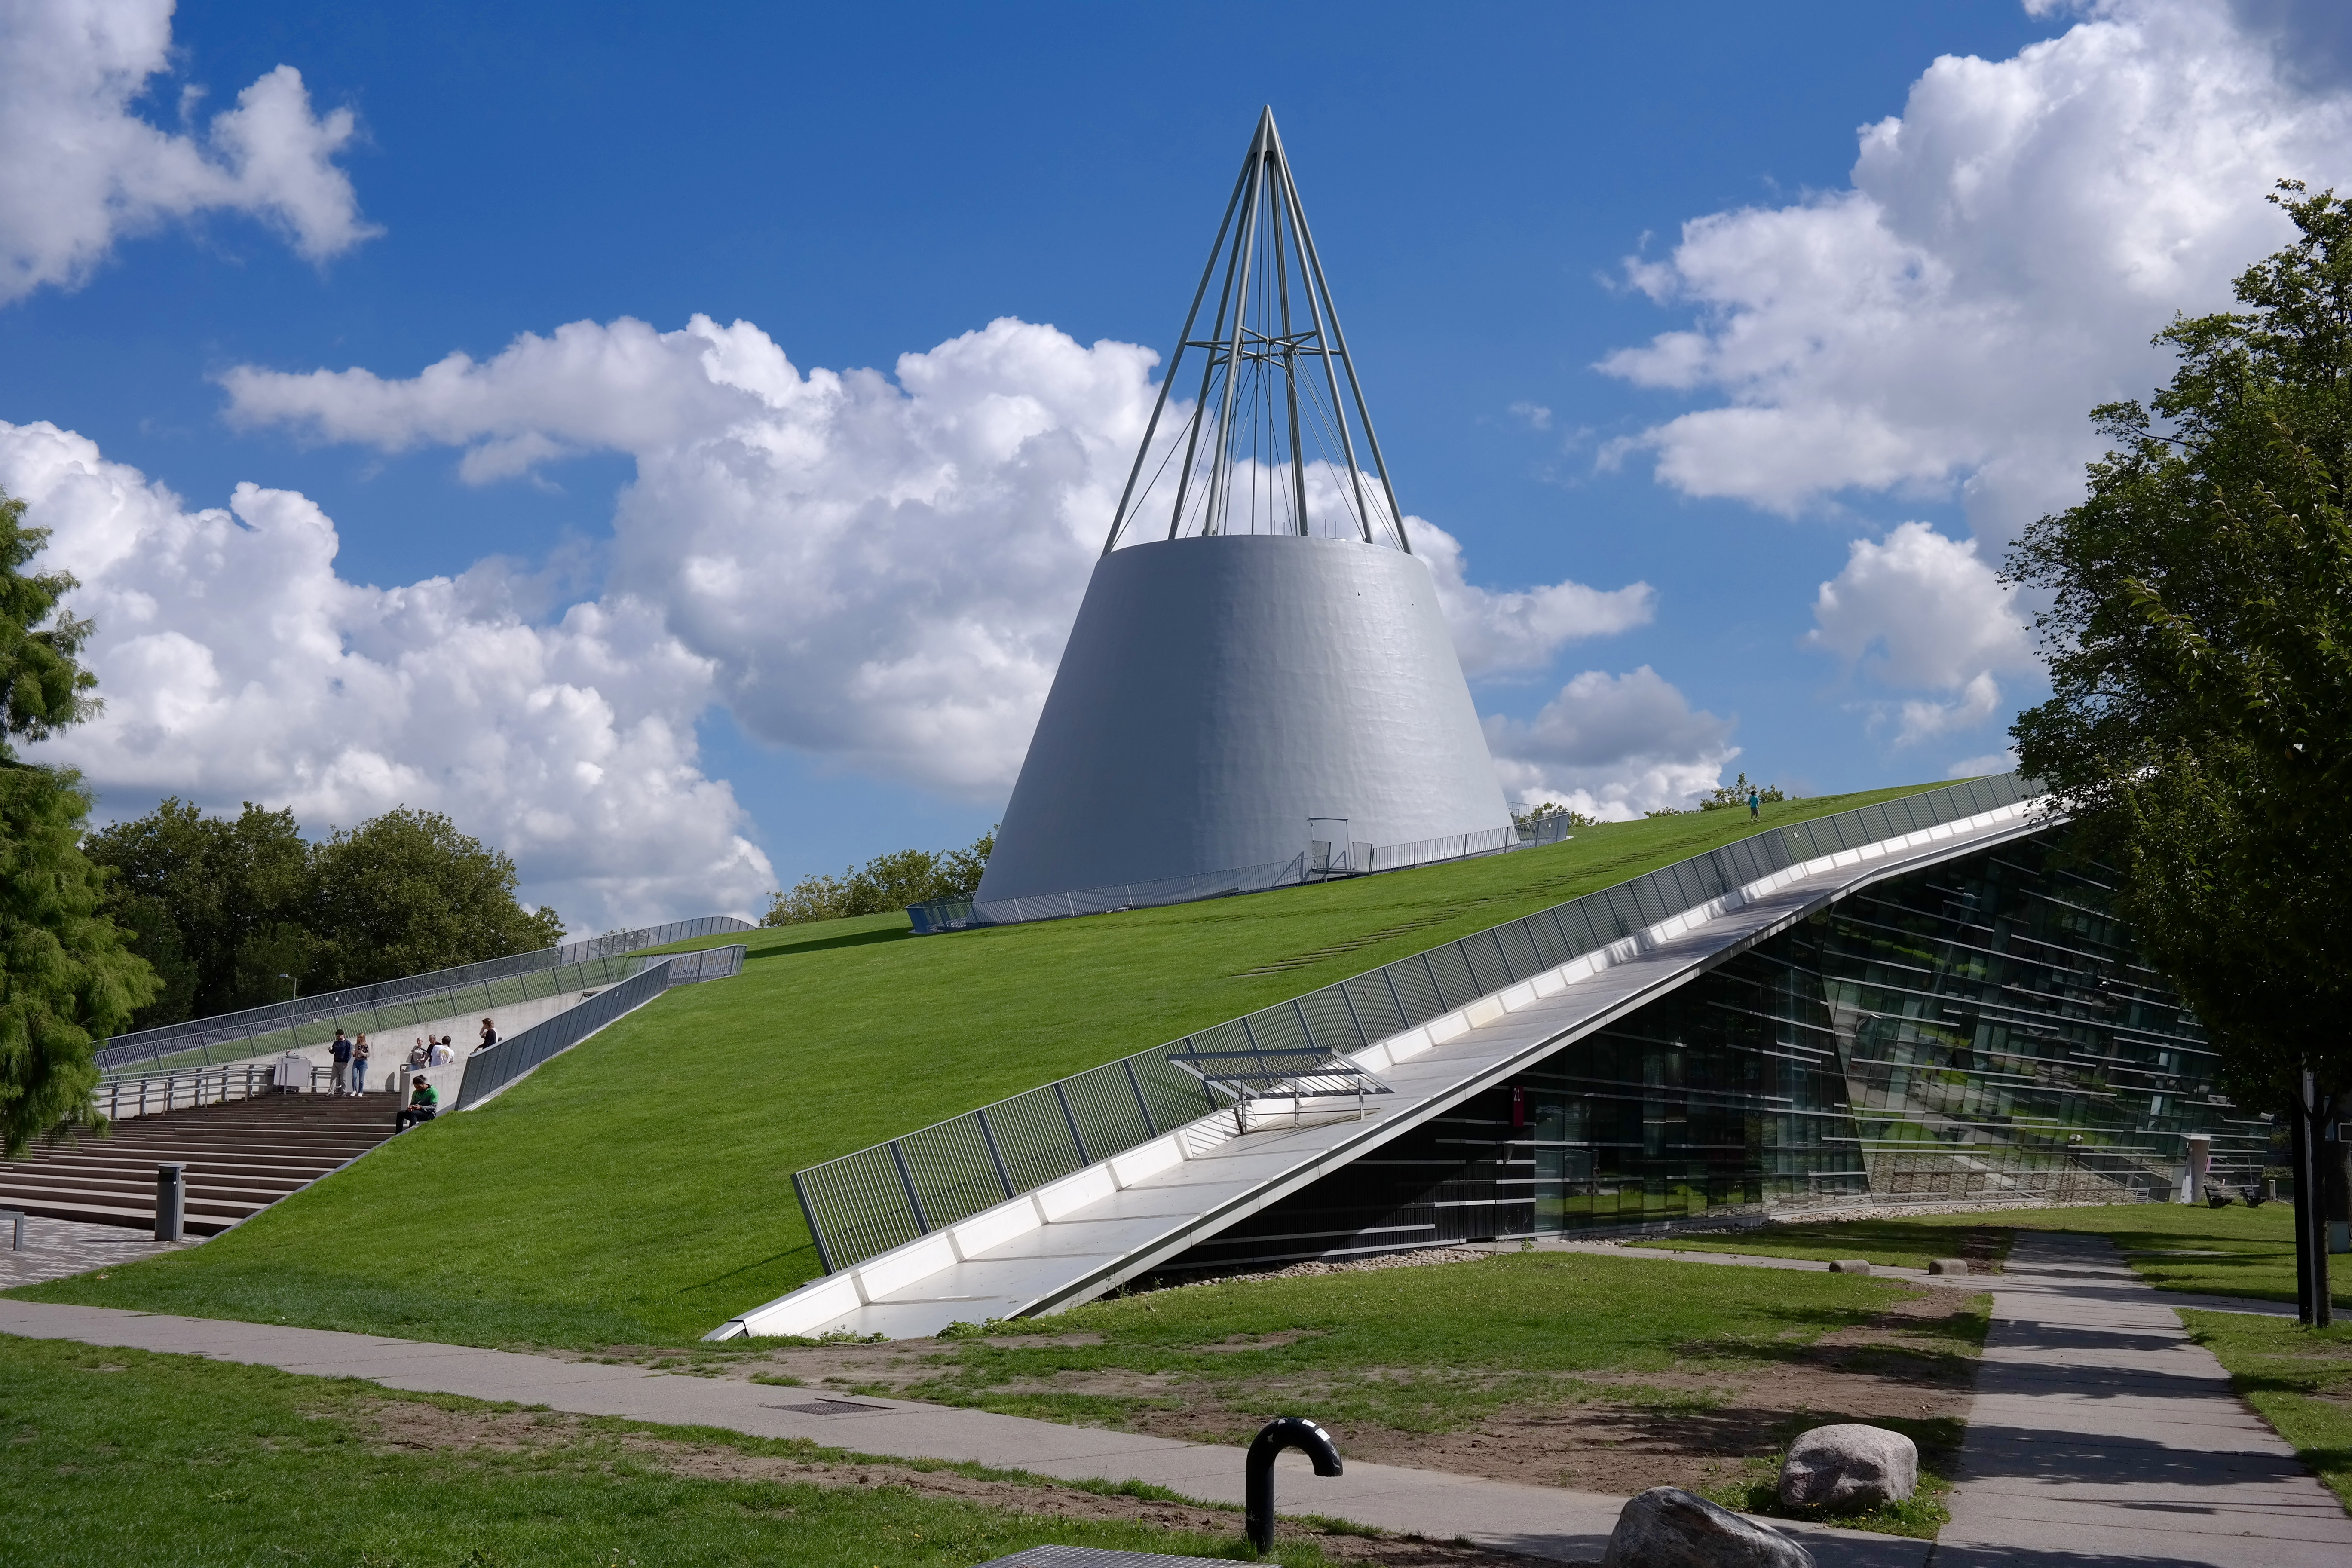
\includegraphics[width=2.1\paperwidth]{figures/Library_TUDelft_sunny.jpg}}}\hfill}
  \section{Full-screen graphics}
}

\begingroup
  \leftfooterwhitetrue
  \rightfooterwhitetrue
  % in case the background does not contrast with the default blue:
  \setbeamercolor{frametitle}{fg=black}
  \usebackgroundtemplate{%
    \hspace*{-0.1\paperwidth}\smash{\raisebox{-1.2\paperheight}{%
      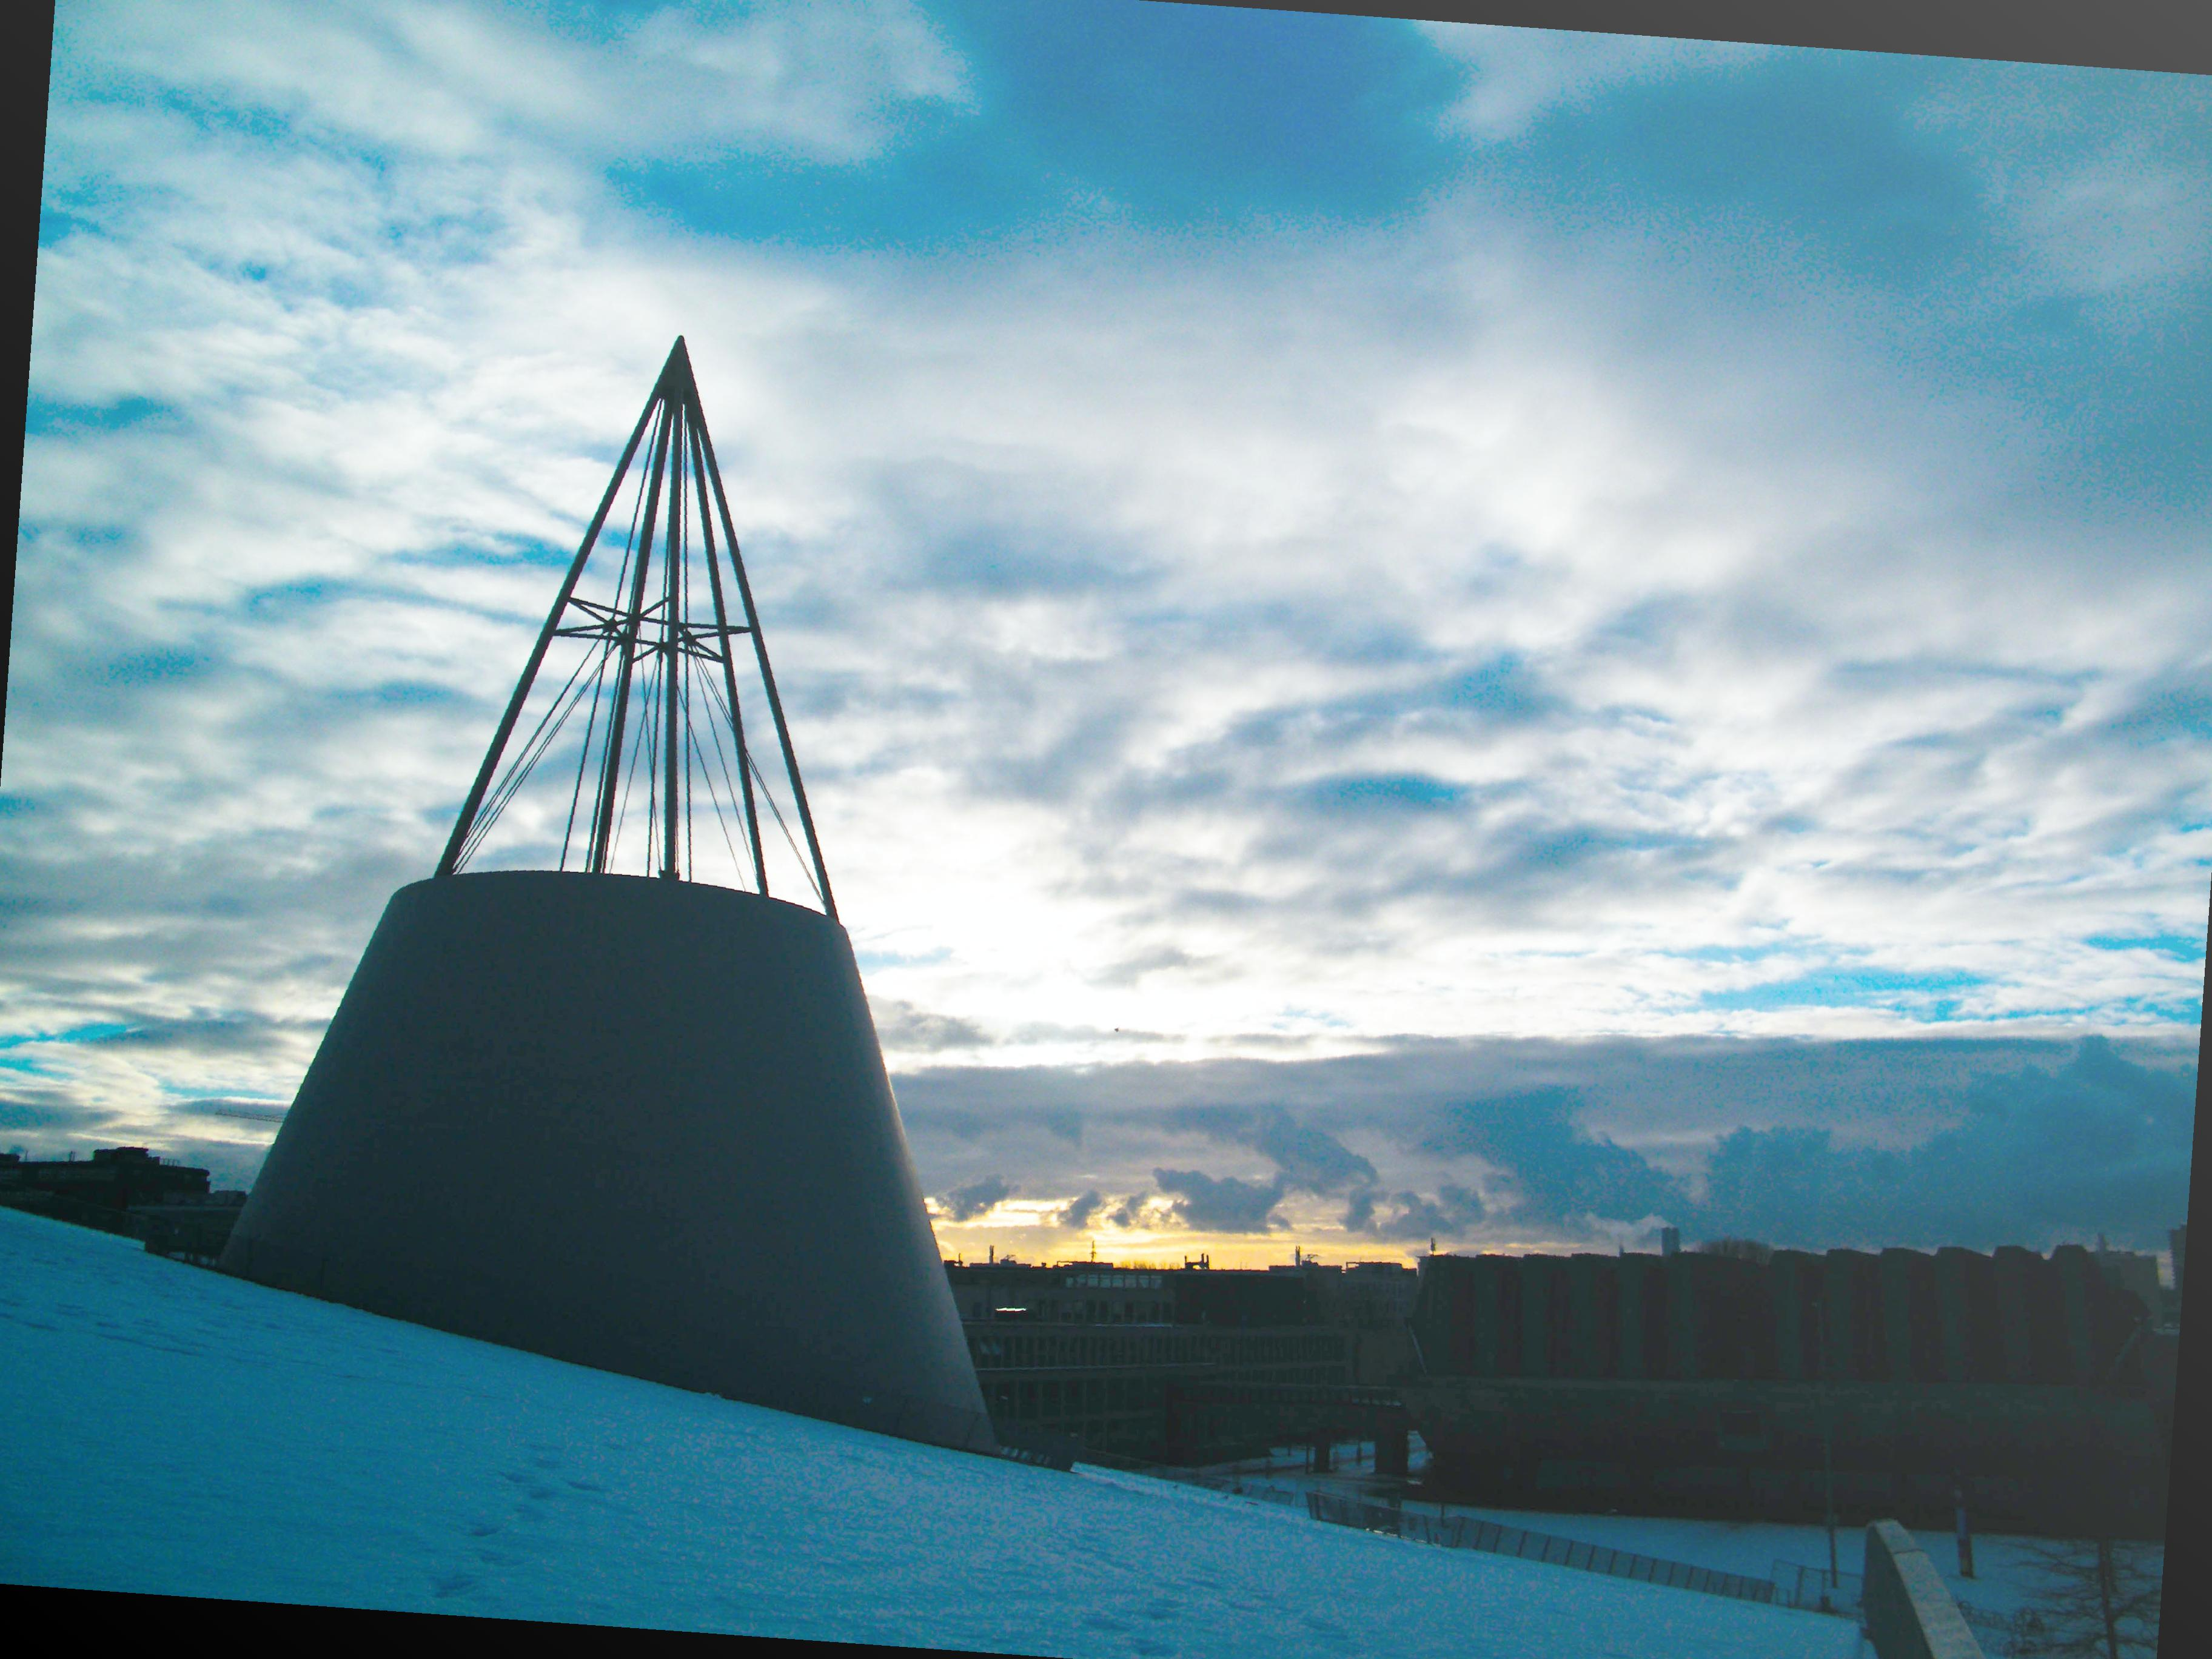
\includegraphics[width=1.2\paperwidth]{figures/Library_TUDelft_sunset_brighter.jpg}}}}%
  \begin{frame}[label=current]{\hfill Sun setting over the TUDelft Library}{\hfill A full-screen graphic}
  \end{frame}
\endgroup

{
  \setlength{\splitpos}{\paperwidth}
  \leftfooterwhitetrue
  \rightfooterwhitetrue
  \renewcommand{\bginsert}{\hspace*{-40ex}\smash{\raisebox{-40ex}{\color{tud RoyalBlue}\tudflame[150ex]}}\hfill}
  \begin{frame}
    \begin{abstikz}
      \node[align=center, font=\color{white}] at (0.5, 0.5)
        {\scalebox{8}{\(E=mc_0^2\)}};
    \end{abstikz}
  \end{frame}
}


{
  \setbeamercolor{frametitle}{fg=white,bg=tud Blue}
  \usebackgroundtemplate{%
    \smash{\hspace*{0\paperwidth}\raisebox{-1.45\paperheight}
      {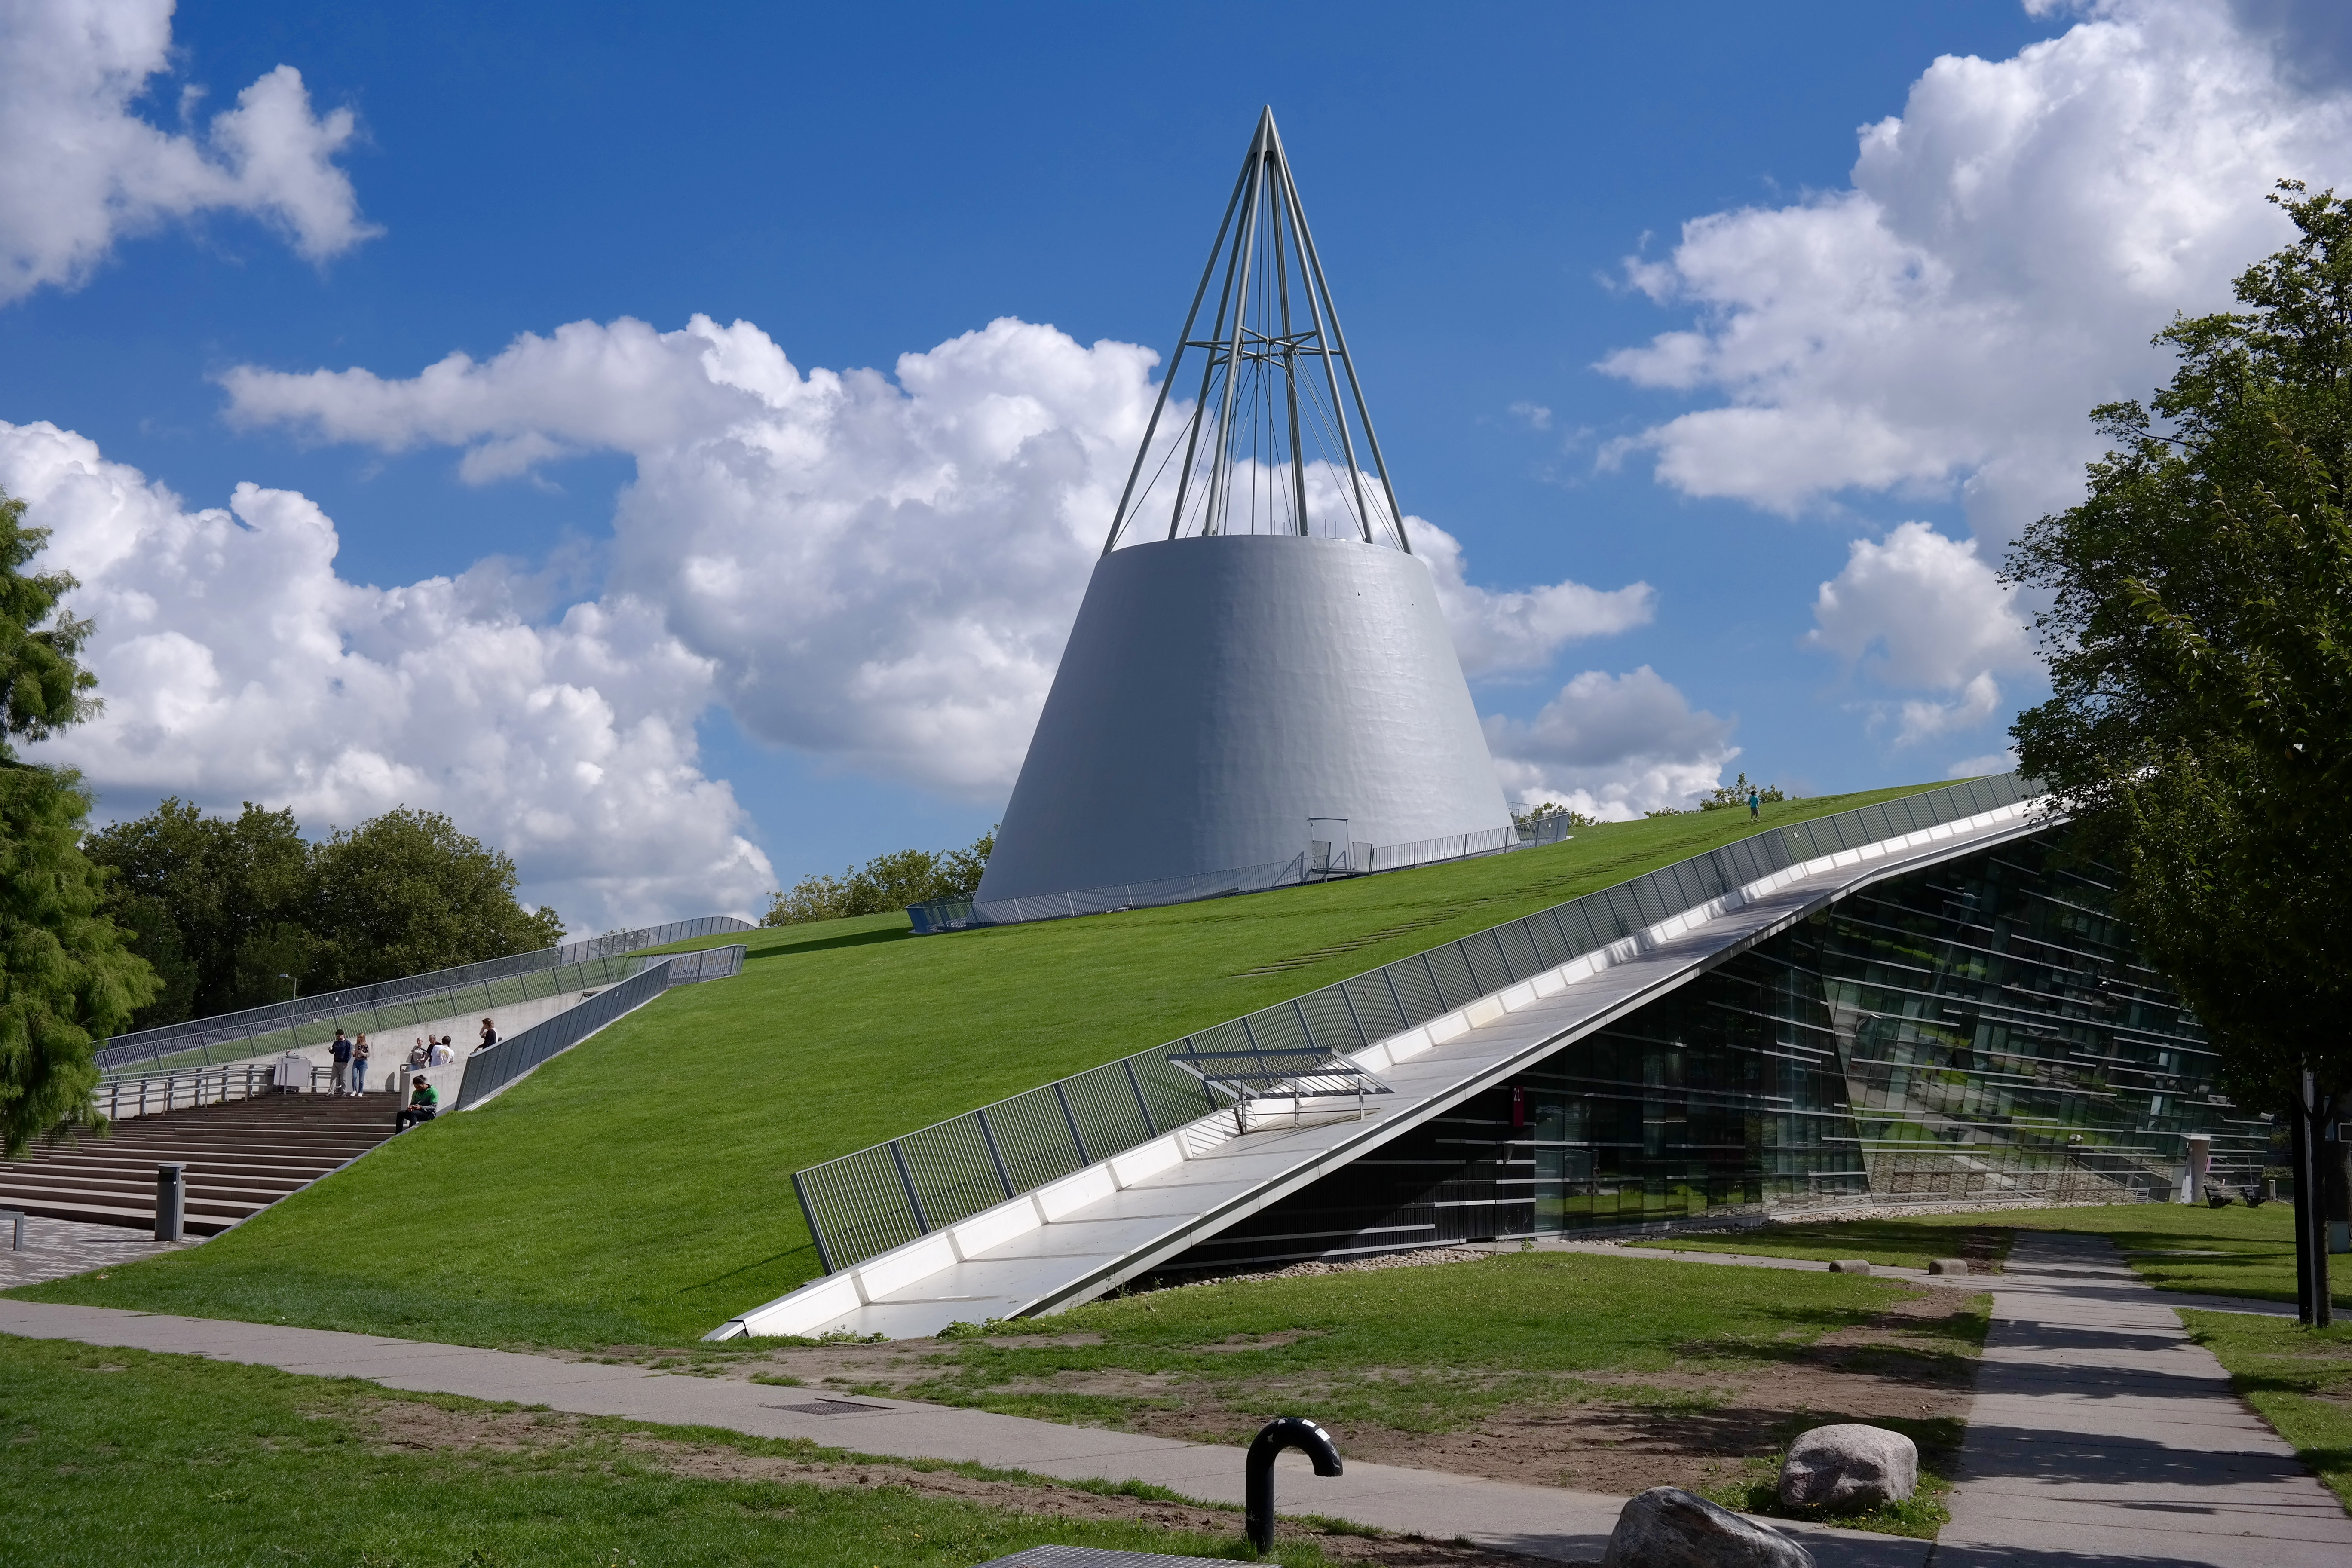
\includegraphics[width=1.1\paperwidth]{figures/Library_TUDelft_sunny.jpg}}}}
  \leftfooterwhitetrue
  \rightfooterwhitetrue
  \begin{frame}
      \frametitle{White Frame Title}
      \framesubtitle{On blue background}
      \textcolor{white}{Optional text\ldots}
  \end{frame}
}